% ENSIBS Assignment
% LaTeX Template
% Version 1.0 (24/12/21)
%
% This template has been downloaded from:
% http://www.LaTeXTemplates.com
%
% Original author:
% WikiBooks (http://en.wikibooks.org/wiki/LaTeX/Title_Creation)
% License: MIT
% 
%----------------------------------------------------------------------------------------
%	PACKAGES AND OTHER DOCUMENT CONFIGURATIONS
%----------------------------------------------------------------------------------------

%\documentclass[a4paper]{article} 
\documentclass[12pt]{article}
\usepackage[french]{babel}
\usepackage[utf8x]{inputenc}
\usepackage{amsmath}
\usepackage{graphicx}
\usepackage{float}
\usepackage{dsfont}
\usepackage{amsfonts}
\usepackage[T1]{fontenc}
\usepackage[colorinlistoftodos]{todonotes}
\usepackage{listings}
\usepackage{geometry}
\newcommand{\deriv}{\mathrm{d}}

\setlength {\marginparwidth}{2cm}

\geometry{hmargin=2.5cm,vmargin=2cm}
\lstset{
    language=R,
    basicstyle=\scriptsize\ttfamily,
    commentstyle=\ttfamily\color{red},
    numbers=left,
    numberstyle=\ttfamily\color{blue}\footnotesize,
    stepnumber=1,
    numbersep=5pt,
    backgroundcolor=\color{white},
    showspaces=false,
    showstringspaces=false,
    showtabs=false,
    frame=single,
    tabsize=2,
    captionpos=b,
    breaklines=true,
    breakatwhitespace=false,
    title=\lstname,
    escapeinside={},
    keywordstyle={},
    morekeywords={}
    }
\title{Projet matière}

\begin{document}

\begin{titlepage}

\newcommand{\HRule}{\rule{\linewidth}{0.5mm}}

\center % Center everything on the page
 
%----------------------------------------------------------------------------------------
%	HEADING SECTIONS
%----------------------------------------------------------------------------------------


\includegraphics[scale=3]{assets/ensibs.png}\\[1cm] % Include a department/university logo - this will require the graphicx package
%\textsc{\Large Computational Statistics}\\[0.5cm] % Major heading such as course name
%\textsc{\large SE331}\\[0.5cm] % Minor heading such as course title

%----------------------------------------------------------------------------------------
%	TITLE SECTION
%----------------------------------------------------------------------------------------

\HRule \\[0.4cm]
{ \huge \bfseries Titre du document
}\\[0.4cm]
\HRule \\[1.5cm]
 
%----------------------------------------------------------------------------------------
%	AUTHOR SECTION
%----------------------------------------------------------------------------------------



\begin{flushleft} \large
\emph{Auteurs :}\\
Prénom \textsc{NOM}\\
Prénom \textsc{NOM}\\
\end{flushleft}

% If you don't want a supervisor, uncomment the two lines below and remove the section above
\Large \emph{Author:}\\
Prenom \textsc{Nom}\\[3cm] % Your name

%----------------------------------------------------------------------------------------
%	DATE SECTION
%----------------------------------------------------------------------------------------

{\large \today}\\[2cm] % Date, change the \today to a set date if you want to be precise

\vfill % Fill the rest of the page with whitespace

\end{titlepage}

\tableofcontents
\newpage

\section{Introduction}
\subsection{Liste}

\begin{enumerate}
\item [$\circ$] Salade
\item [$\circ$] Tomate
\item [$\circ$] Ognion
\end{enumerate}

\subsection{Image}

\begin{figure}[htp!]
  \centering
  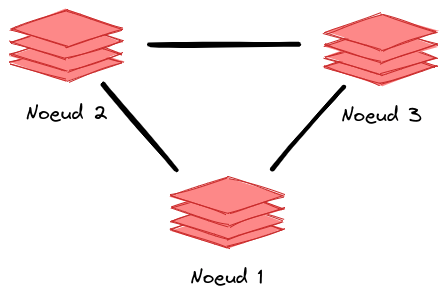
\includegraphics[width=1\textwidth]{assets/screenshots/noeuds.png}
  \caption{Plan d'adressage}
  \label{fig:figure1}
\end{figure}

\section{Conclusion}

La conclusion

\end{document}